\documentclass{scrreprt}
\usepackage[margin=0.7in]{geometry} %réduire marges

\setkomafont{disposition}{\normalfont\bfseries}

%french
\usepackage[utf8]{inputenc}
\usepackage[colorlinks=true,urlcolor=blue,linkcolor=blue]{hyperref}
\usepackage[T1]{fontenc}
\usepackage[francais]{babel} %en Français
\usepackage[pdftex]{graphicx}
\usepackage{listings}
\usepackage{color}
\definecolor{mygreen}{rgb}{0,0.6,0}
\lstset{language=C++,
  basicstyle=\ttfamily,
  keywordstyle=\color{blue}\ttfamily,
  stringstyle=\color{red}\ttfamily,
  commentstyle=\color{mygreen}\ttfamily,
  morecomment=[l][\color{brown}]{\#},
  morecomment=[l][\color{violet}]{\#define},
  breaklines=true
}

\usepackage{graphicx} %pour les images

\usepackage{xcolor}

\setcounter{tocdepth}{3}
\definecolor{Zgris}{rgb}{0.87,0.85,0.85}

\newsavebox{\BBbox}
\newenvironment{DDbox}[1]{
\begin{lrbox}{\BBbox}\begin{minipage}{\linewidth}}
{\end{minipage}\end{lrbox}\noindent\colorbox{Zgris}{\usebox{\BBbox}} \\
[.5cm]}


\begin{document}
\title{Projet PERI}
\subtitle{\textit{Rapport}}
\date{26 mai 2015}
\author{Maxime \textsc{Bittan}, Daniel \textsc{Bourdrez}, Redha \textsc{Gouicem},\\ Alexandra \textsc{Hospital}, Ilyas \textsc{Toumlilt}}


\maketitle

\pagebreak
\tableofcontents

\pagenumbering{arabic}

Dans ce (pas très) court tutoriel, nous allons vous montrer comment 
fabriquer votre propre station météo. Et comme ça serait un peu trop banal, 
votre station météo sera en plus mobile ! Nous proposons pour cela une
architecture assez simple, avec d'un côté une Raspberry Pi qui fera office de
serveur et de gestionnaire, et d'un autre côté une Arduino motorisée faisant
office de station météo.

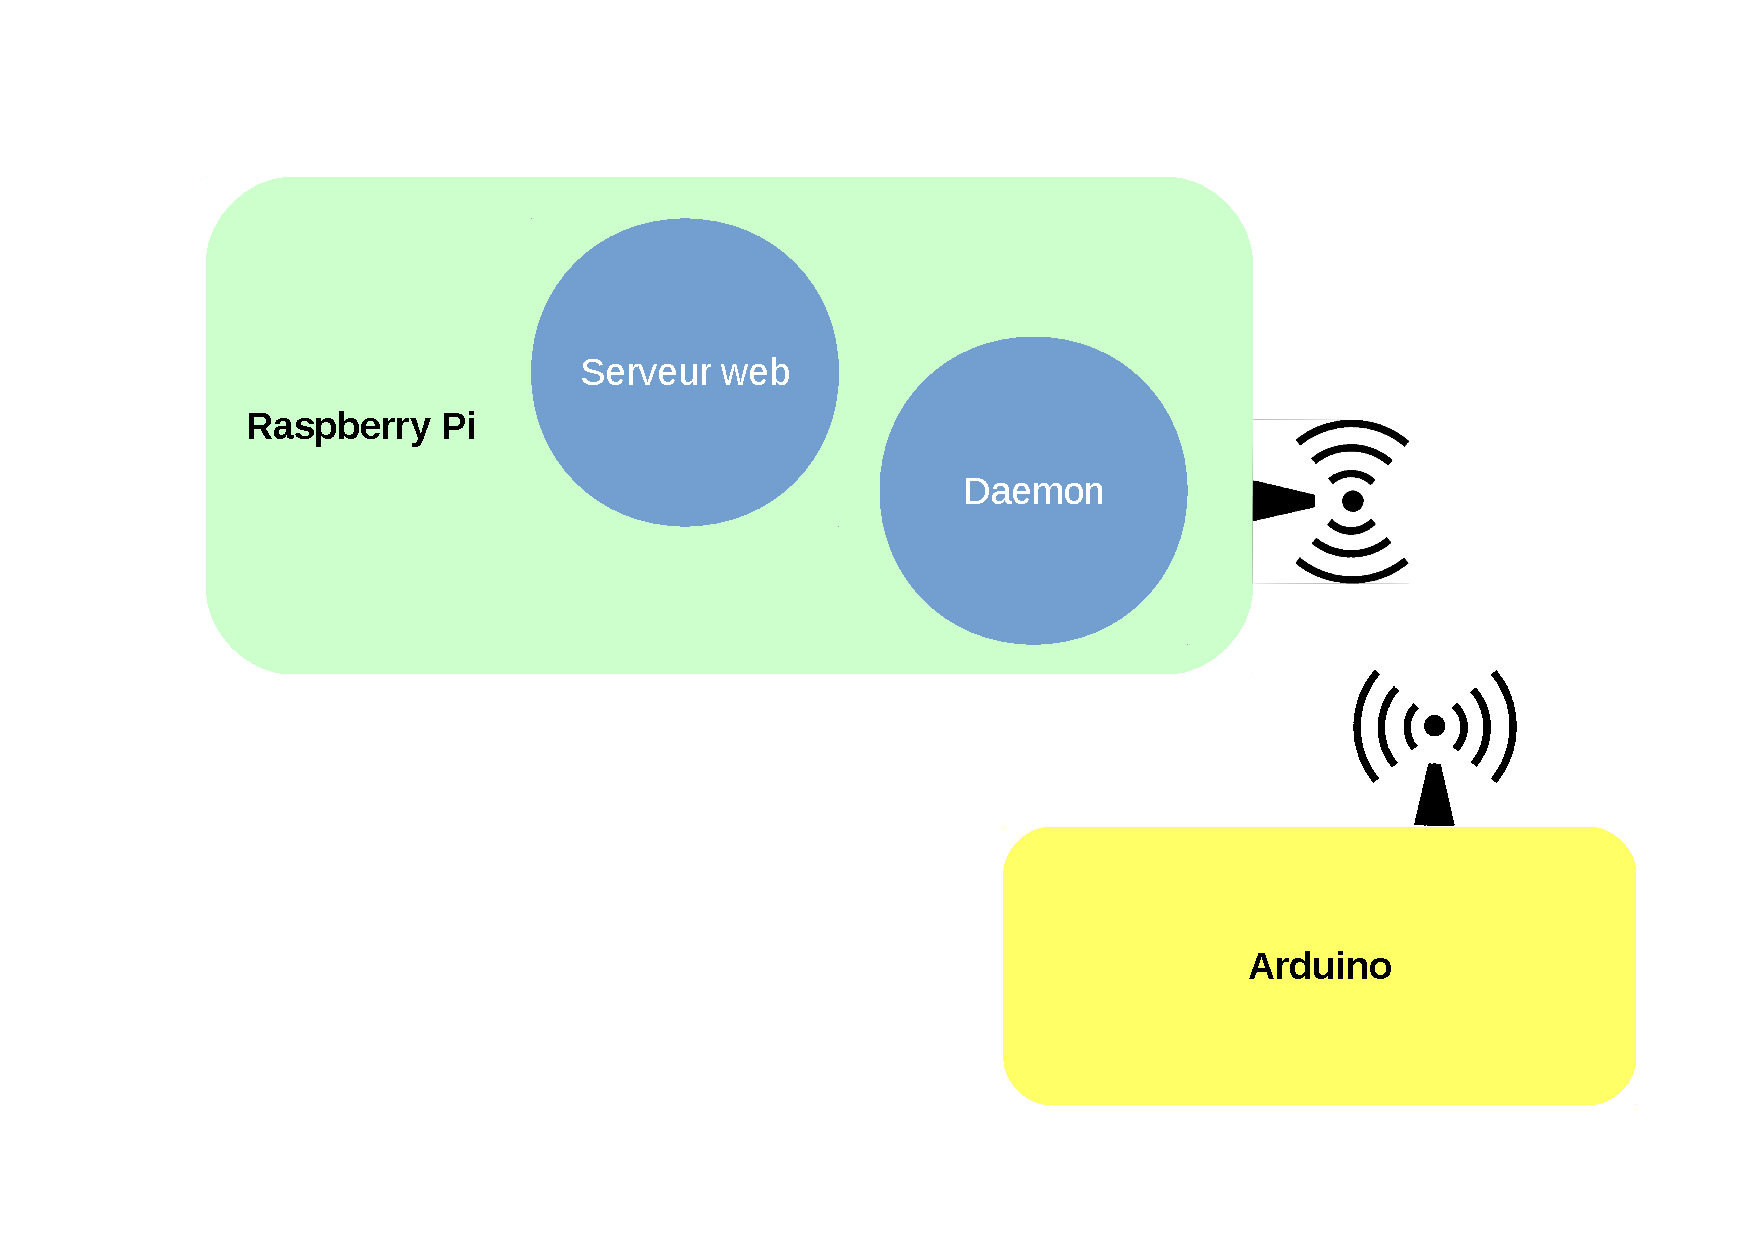
\includegraphics[width=\textwidth]{include/archi.pdf}

On notera que la Raspberry contient deux entités : le serveur web, qui permettra
de tout gérer de l'extérieur, et le daemon, qui fera le lien entre le serveur 
web et l'Arduino par le biais de communications radios.


\chapter{Montage matériel}
\label{ch:montage}
Afin de réaliser notre station météo mobile, nous avons deux montages à
réaliser :
\begin{itemize}
\item le serveur (Raspberry Pi)
\item la station mobile (Arduino motorisée)
\end{itemize}

\section{Serveur}

\section{Station mobile}
Le montage sera le suivant :
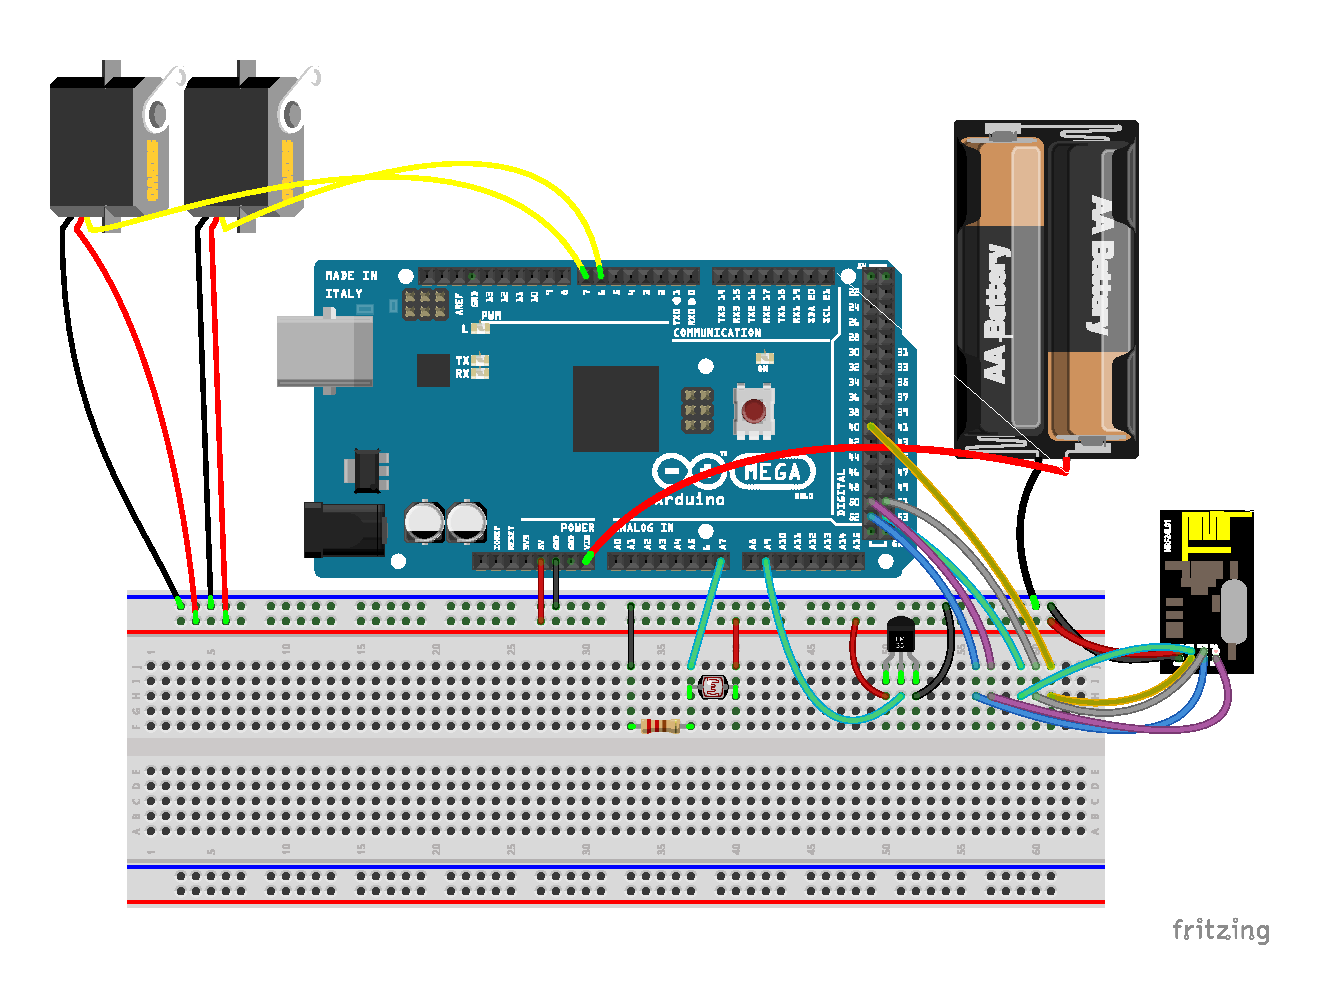
\includegraphics[scale=0.5]{include/arduino_bb.pdf}
\paragraph{}
On ne parlera pas ici de l'aspect mécanique (chassis, placement des moteurs,
etc...).


\chapter{Serveur}
Exécuté sur la Raspberry Pi, sollicité par un ( ou plusieurs ) client(s) d’un côté et un ( ou plusieurs ) démon(s) de l’autre. Le serveur web est la pièce maîtresse de ce projet, il doit pouvoir servir toutes les requêtes, en continu, tout en assurant la cohérence des données transitantes, leur fiabilité, ainsi qu’une gestion intelligente de la mémoire ( les requêtes pouvant facilement atteindre un nombre très considérable ). Nous reviendrons plus en détails sur la nature de ces requêtes ainsi que les implémentations choisies.

\section{Choix de l'environement}

\subsection{Le serveur HTTP}

Entre de simples scripts sh/python en CGI, un NodeJS plus flexible mais peu fiable, nous avons décidé de jouer la carte de la performance - et de l’enchevêtrement aussi, je l’assume - et nous choisîmes donc l’\textbf{Apache2}.\\
Ce serveur HTTP, l’un des plus populaires du World Wide Web, est spécialement adapté pour les environnements UNIX, une harmonie dont nous profiterons pleinement, vu que notre Raspberry Pi tourne sous Linux. Apache2 est également conçu pour prendre en charge de nombreux modules lui donnant des fonctionnalités supplémentaires, nous en utiliserons les suivantes :
\begin{itemize}
\item Interprétation du langage PHP.
\item Serveur Proxy, nécessaire pour l’exécution sur l’environnement de la fac ( ARI alias PPTI ).
\item Common gateway interface.
\item Server sides includes.
\item La réécriture d’URLs.
\item Et quelques protocoles de communication additionnels.
\end{itemize}
( Nous reviendrons sur l’utilisation de ces fonctionnalités quand nous commencerons à voir leur implémentation )

\subsection{Choix des langages}

L’adoption d’Apache2 nous permet donc un choix très large au niveau des langages, cependant, PHP reste le langage le mieux interprété par ce serveur HTTP.\\
PHP est un langage de script, utilisé le plus souvent côté serveur. Dans notre architecture, le serveur Apache2 interprète le code PHP des pages Web ou des scripts demandés et génère du code (HTML, XHTML, CSS par exemple) et des données (JPEG, GIF, PNG par exemple) pouvant être interprétées et rendues par un navigateur web.\\
Autre sa souplesse, PHP nous permettra une gestion assez ``bas niveau'' ( par rapport à ses concurrents, dans le domaine ) de notre serveur Web et de ses protocoles, il implémente également toute la bibliothèque POSIX dont nous allons nous servir pour relayer les données au démon.\\
Un dernier avantage de PHP, et sûrement le plus pertinent, et son côté ``dynamique'' ( ce qui fait majoritairement son succès et son adoption par des géants comme Google, Facebook … ). Une page web dynamique ( par opposition à une page web statique ), et une page dont le contenu peut varier en fonction des informations qui ne sont connues qu’au moment de sa consultation, mieux le contenu de ces pages peut même varier après le chargement et au cours du temps, sans avoir à recharger la page, pour cela nous aurons besoin de définir une méthode de dialogue, entre le navigateur client, et le serveur.\\
\\
Avant de définir cette méthode, nous avons besoin de définir les langages côté client, pour ce côté, on restera dans le classique, HTML + CSS pour l’affichage de la page, et de JavaScript ( JS, JQuery et DOM ) pour les scripts client.
\\
La méthode de dialogue entre le client et le serveur sera donc AJAX, qui permet de construire des sites web dynamique et interactifs, dans notre cas cette communication se fera essentiellement en manipulant des XMLHttpRequest, ainsi :
\begin{itemize}
\item DOM et JavaScript permettent de modifier l'information présentée dans le navigateur en respectant sa structure
\item l'objet XMLHttpRequest sert au dialogue asynchrone avec le serveur Web
\item XML structure les informations transmises entre serveur Web et navigateur.
\end{itemize}

\subsection{Installation de l'environnement}

Afin que tout cela fonctionne, il est nécessaire d’installer quelques outils, le script ./web/install\_env.sh contient les commandes bash nécessaires :\\

\begin{DDbox}{\linewidth}
\begin{lstlisting}[language=bash]
        sudo aptitude update
        sudo aptitude upgrade
        sudo aptitude install apache2
        sudo aptitude install php5
        sudo aptitude install mysql-server php5-mysql
        sudo rm /var/www/index.html
        echo "<?php phpinfo(); ?>" > /var/www/index.php
\end{lstlisting}
\end{DDbox}
\\
Vous l’aurez donc compris, les sources php doivent se trouver dans /var/www/ pour être interprétées, chemin dont le point d’entrée est http://localhost/ , depuis un navigateur web.


\section{Conception du serveur Web}

De manière plus conceptuelle, le client a besoin de pouvoir générer la page web depuis son navigateur ( nous reviendrons sur les composants de cette page ) et donc y avoir un accès par URL, cette adresse devrait mener, du point de vue de notre projet, au point d’entrée du serveur, c’est à dire dans le cas d’un serveur php, le fichier index.php placé à la racine du projet.\\
Le client aura ensuite besoin de transmettre des commandes asynchrones et dynamiques pour modifier les données sur son interface ou pour donner des ordres ( commandes ) au serveur, pour cela nous utiliserons le protocole AJAX décrit plus haut.\\
Finalement, et d’un autre côté, le démon utilisera, pour ses communications avec le serveur des pipes fifo Posix.

\section{Retour sur la station météo mobile}

Maintenant que l’environnement, langages et protocoles ont été définis, nous pouvons y refléter le but de notre projet, en effet, contrôler la voiture signifie envoyer des commandes vers celle-ci, le client devrait donc pouvoir, à l’aide de la page web générée, envoyer des commandes asynchrones, contrôlant la vitesse ou l’orientation, cette commande, et comme présenté plus haut, sera relayée grâce à l’AJAX qui va réveiller un script cible sur le serveur destiné à traiter cette commande, dans notre cas, l’écriture d’une commande correspond à son transfert sur le pipe du démon. Une autre partie du projet consiste à recueillir les informations relatives à la température et luminosité pour les afficher sur la page web, pour cela les scripts serveur devront lire sur le pipe démon qui fournira ces données, et les écrire sur les champs dédiés de l’interface, en passant encore par le moyen de communication asynchrone, AJAX.

\section{La page web principale - IHM}

Générée à la demande par l’utilisateur depuis un URL, elle se compose d’une interface web ( HTML + CSS ), et d’un ensemble de scipts JavaScript permettant le dynamisme et implémentant en utilisant JQuery et DOM, l’IHM ( Interface Homme-Machine ).

\subsection{Les bibliothèques utilisées}

Tant utiles pour l’ergonomie que pour leur facilité d’utilisation, les bibliothèques graphiques ( ou CssLibs pour les HTMLiens ) nous offrent des avantages très considérables dont nous allons profiter, le but est simple : avoir une interface simple, jolie et réactive, sans coder une seule ligne pour l’implémenter.\\
Ces librairies se trouvent dans ./web/lib/\\
\\
\textbf{Twitter Boostrap :}\\
Très connu pour la création de sites et d’applications web, bootstrap est une collection d’outils contenant des codes HTML et CSS, des formulaires, boutons et autres éléments interactifs, ainsi que des extension JavaScript en option.
\\
\textbf{Extended Bootstrap:}\\
Une version étendue de Bootstrap, que j’ai développé moi-même l’été dernier et qui contient un ensemble de scripts ( js ) permettant d’avoir des pages web en responsive design, version mobile mais surtout surcouchant la classe plot, permettant de dessiner des graphes et schéma, dont on va nous servir pour éviter de passer par google charts.\\
Une documentation en version html de cette lib est disponible dans ./web/lib/doc/\\
\\
\textbf{Jquery :}\\
Une biblithèque javascript permettant de parcourir et modifier le DOM ( arbre syntaxique de la page HTML ) et la gestion des événements et de effets visuels.\\
\\
On va donc commencer par inclure toutes ses libs dans notre page HTML :\\
\\
Les CSS dans les headers :\\
\begin{DDbox}{\linewidth}
\begin{lstlisting}[language=html]
  <link rel='stylesheet' media='all' type='text/css' href='./lib/bootstrap-3.3.4/dist/css/bootstrap.css' />
	 <!-- extended bootstrapCss -->
	 <link href="lib/extendedBootstrap/css/bootstrap.min.css" rel="stylesheet" />
	 <link href="lib/extendedBootstrap/css/font-awesome.min.css" rel="stylesheet" />

	 <link rel="stylesheet" href="lib/extendedBootstrap/css/jquery-ui-1.10.3.custom.min.css" />
	 <link rel="stylesheet" href="lib/extendedBootstrap/css/chosen.css" />
	 <link rel="stylesheet" href="lib/extendedBootstrap/css/datepicker.css" />
	 <link rel="stylesheet" href="lib/extendedBootstrap/css/bootstrap-timepicker.css" />
	 <link rel="stylesheet" href="lib/extendedBootstrap/css/colorpicker.css" />
	 <link href="lib/extendedBootstrap/css/refineslide.css" rel="stylesheet" />
	 <link href="lib/extendedBootstrap/css/bootstro.css" rel="stylesheet" />

	 <link rel="stylesheet" href="lib/extendedBootstrap/css/jquery-slider.css" />
	 <link rel="stylesheet" href="lib/extendedBootstrap/css/checkbox-radio-switch.css" />
	 <link href="lib/extendedBootstrap/css/extend.css" rel="stylesheet" />
\end{lstlisting}
\end{DDbox}
\\
Et les JS à la fin du body juste avant de fermer </body> :\\
\begin{DDbox}{\linewidth}
\begin{lstlisting}[language=html]
  <script src="lib/extendedBootstrap/js/bootstrap.min.js"></script>
      <script src="lib/extendedBootstrap/js/jquery-ui-1.10.3.custom.min.js"></script>

      <script src="lib/extendedBootstrap/js/flot/jquery.flot.min.js"></script>
      <script src="lib/extendedBootstrap/js/flot/jquery.flot.pie.min.js"></script>
      <script src="lib/extendedBootstrap/js/flot/jquery.flot.resize.min.js"></script>

      <script src="lib/extendedBootstrap/js/date-time/bootstrap-datepicker.min.js"></script>
      <script src="lib/extendedBootstrap/js/date-time/bootstrap-timepicker.min.js"></script>
      <script src="lib/extendedBootstrap/js/bootstrap-colorpicker.min.js"></script>

      <script src="lib/extendedBootstrap/js/jquery.knob.min.js"></script>
      <script src="lib/extendedBootstrap/js/jquery.autosize-min.js"></script>
      <script src="lib/extendedBootstrap/js/jquery.inputlimiter.1.3.1.min.js"></script>
      <script src="lib/extendedBootstrap/js/jquery.maskedinput.min.js"></script>
      <script src="lib/extendedBootstrap/js/jquery.refineslide.js"></script>
      <script src="lib/extendedBootstrap/js/bootbox.js"></script>
      <script src="lib/extendedBootstrap/js/bootstro.min.js"></script>
\end{lstlisting}
\end{DDbox}

\subsection{Architecture de la page principale}

La page principale se compose de trois champs majeurs :
\begin{itemize}
\item Control de la voiture
\item Temperature
\item Luminosité
\end{itemize}

Ces champs sont des balises div, dont l’attribut id identifie de manière unique chacun des 3 :\\
\begin{DDbox}{\linewidth}
\begin{lstlisting}[language=html]
  <div id='carControlContainer' >

  </div>
  
  <div id='temperatureContainer' >

  </div>

  <div id='graphContainer' >

  </div>
\end{lstlisting}
\end{DDbox}
\\
Le corps de chaque composant sera représenté par un panel Bootstrap, dont la structure est la suivante :\\
\begin{DDbox}{\linewidth}
\begin{lstlisting}[language=html]
  <div class="panel panel-default">
	    <div class="panel-heading">
	       <h3 class="panel-title">
		  ICI LE TITRE DU PANEL
	       </h3>
	    </div>
	    <div class="panel-body">
	       ICI LE CORPS DU PANEL
	    </div>
	 </div>
\end{lstlisting}
\end{DDbox}
\\
Bootstrap et ExtendedBoostrap s'occupent de gérer la mise en forme et la mise en page selon la taille de la fenêtre, il suffit par exemple ici de leur indiquer l'attribut class d'une balise pour qu'ils sachent ce qu'il faut faire.
\\
\\
A partir de là, à chaque fois que nous parlerons du contenu d'une section, on fera directement référence au corps du panel.

\subsection{Car control}

Dans cette partie, nous avons besoin d'interactions à double-sens, c’est à dire, et avoir des objets cliquables pour envoyer nos commandes, et pouvoir afficher l’été actuel de ces valeurs, on a donc opté pour des barres deux barres de défilement, une pour contrôler la vitesse de la voiture et une autre pour contrôler son orientation, les deux barres son munies de deux flèches pour chaque extrémité permettant d’incrémenter/décrémenter les valeurs.\\
Le changement des valeurs et la gestion du clique seront traitées ultérieurement.

\subsection{Weather station}

Cette partie ne fait qu'afficher en texte brut la valeur de la température.

\subsection{Brightness graph}

La partie la plus compliquée graphiquement, elle contient le graphe qui devrait afficher en temps-réel les valeurs de luminosité reçues. Ce graphe est représenté par un canvas où on commence par dessiner les deux axes et les légendes, puis une fois l’ensemble créé, un fichier js intervient, il s’agit de :\\
\begin{DDbox}{\linewidth}
\begin{lstlisting}[language=html]
<script src='./js/charts-flot.js'></script>
\end{lstlisting}
\end{DDbox}
\\
Ce fichier définit quelques fonctions essentielles à la gestion du graphe, la partie qui nous intéresse ici est contenue dans
\begin{lstlisting}[language=java]
  $(document).ready{}
  \end{lstlisting}
et qui veut dire ``exécute mon corps au chargement de la page'', cette partie contient un tableau de donnée data, qu’on initialise de la sorte :\\
\begin{DDbox}{\linewidth}
  \begin{lstlisting}[language=java]
  function initChart() {
      for(var i = 0; i < totalPoints; i++){
	 data.push(0);
	 res.push([i, 0]);
      }
      
      return res;
   }
\end{lstlisting}
\end{DDbox}
\\
( res étant une hashmap associant à chaque point de l’axe des y, une valeur data correspondante )
Nous passons ensuite à l’initialisaion du plot :\\
\begin{DDbox}{\linewidth}
\begin{lstlisting}[language=java]
  var plot = $.plot($("#realtimechart"), [initChart()], options);
\end{lstlisting}
\end{DDbox}
\\
et à un premier dessin :\\
\begin{DDbox}{\linewidth}
\begin{lstlisting}[language=java]
  plot.setData([res]);
plot.draw();
\end{lstlisting}
\end{DDbox}
\\
La suite est donc intuitive, à chaque réception de donnée, on la rajoute au tableau data et on update le chart :\\
\begin{DDbox}{\linewidth}
\begin{lstlisting}[language=java]
  function updateChart(newValue) {
      if( data.length > 0)
	 data = data.slice(1);
      
      data.push(newValue);
      
      // zip the generated y values with the x values
      res = [];
      for(var i = 0; i < data.length; i++){
	 res.push([i, data[i]]);
      }
      
   }
\end{lstlisting}
\end{DDbox}

\section{L'interface AJAX}

Gère les communication entre le client et le serveur, composée de fichier javascripts côté client et de scripts PHP côté serveur, nous allons commencer par inclure nos fichiers js sur la page principale :\\
\begin{DDbox}{\linewidth}
\begin{lstlisting}[language=html]
  <script src='./ajax/ajax.js'></script>
	 <script src='./js/charts-flot.js'></script>
	 <script src='./js/speedUp.js'></script>
	 <script src='./js/turn.js'></script>
	 <script src='./js/temperature.js'></script>
\end{lstlisting}
\end{DDbox}
\\
Le premier ( ajax.js ) implémente les fonctions permettant d'envoyer nos requêtes HTTP vers le serveur, on utilise une instance la classe XMLHTTPRequest(), à la quelle on associe l'URL cible et la fonction js cible à appeler en cas de réponse, ansi que les données à envoyer sous forme de paramètres en POST. Le corps de la fonction est simple, et nous donne :\\
\begin{DDbox}{\linewidth}
\begin{lstlisting}[language=java]
  function ajax_brightness(url, flux, rappel, arg, method) {
  var r = window.XMLHttpRequest ? new XMLHttpRequest() :
    (window.ActiveXObject ?  new ActiveXObject("Microsoft.XMLHTTP") : '');
  if (!r) return false;
  r.onreadystatechange = function () {rappel(r, arg);};
  r.open(method ? method : 'POST', url, true);
  if (flux)
      r.setRequestHeader("Content-Type", 
                         "application/x-www-form-urlencoded; ");
  r.send(flux);
  return true;
}
\end{lstlisting}
\end{DDbox}
\\
Les autres fichiers contiennent justement ces fonctions de rappel, en plus des fonctions de déclenchement ( par timeout ou par clique selon le besoin ) des requêtes AJAX.\\
Prenons pour exemple la temperature, le fichier temperature.js se charge de gérer le champ température, chaque seconde il fait appel à :\\
\begin{DDbox}{\linewidth}
\begin{lstlisting}[language=java]
var temperatureUpdateInterval = 1000;
   function updateTemperature() {
      if( !tempLock ){
	 tempLock = 1;
	 document.getElementById("temperatureLoading").style.display = "initial";
	 ajax_temperature("./ajax/temperatureAjax.php", 0, receiveTemperature, 0);
      }
      setTimeout(updateTemperature, temperatureUpdateInterval);
   }
\end{lstlisting}
\end{DDbox}
\\
cette fonction s'occupe d'appeler, en passant par le script ajax, le script PHP serveur temperatureAjax.php, qui se charge lire dans le pipe et renvoyer en texte brut la valeur de la temperature ( ou des erreurs en cas de non présence du démon, ou de mauvaise requête ) :

\begin{DDbox}{\linewidth}
\begin{lstlisting}[language=php]
<?php

define('TEMP_FIFO', "/tmp/temppipe");

$ret = "";

if(!file_exists(TEMP_FIFO)){
   $ret = "ERROR 030: Daemon isn't lunched yet";
   goto end_label;
}

$pipe = fopen(TEMP_FIFO, "r");
if( !$pipe ){
   $ret = "ERROR 031: Cannot open TEMP_FIFO pipe";
   goto end_label;
}

$ret = ord(fread($pipe, 2));

fclose($pipe);

end_label:
   header("Content-type: text/plain;charset=utf-8");
   echo $ret;
\end{lstlisting}
\end{DDbox}
\\
Une fois la valeur retournée, la fonction de rappel est appelée :\\
\begin{DDbox}{\linewidth}
\begin{lstlisting}[language=java]
  function receiveTemperature(xhr, arg){
      if (xhr.readyState === 4) {
	 if (xhr.status === 200) {
	    if (xhr.responseText) {
	       if (/^Error/.test(xhr.responseText)) {
		  alert(xhr.responseText);
	       } else {
		  /* Si on est le c est que la reponse est bonne */
		  tempVal = parseInt(xhr.responseText);
		  updateTemperatureField();
		  tempLock = 0;
		  document.getElementById("temperatureLoading").style.display = "none";
	       }
	    } else {
	       alert("ERROR: response is not valid");
	    }
	 }
      }
   }  
\end{lstlisting}
\end{DDbox}
\\
Remarque, la fonction updateTemperatureField() utilise l'arbre syntaxique DOM pour modifier le contenu de la balise temperature :\\
\begin{DDbox}{\linewidth}
\begin{lstlisting}[language=html]
  function updateTemperatureField()
   {
      document.getElementById("temperatureValue").innerHTML = tempVal;
   }
\end{lstlisting}
\end{DDbox}

\subsection{Synchronisation}

Pour assurer la réactivité de la page, et pour éviter l'empilement inutile des commandes, une synchronisation entre le client et le serveur s'impose, on se fixe comme règle de ne jamais envoyer une deuxième requête, tant que la première n'a pas été satisfaite, pour celà j'ai utiliser un système de lock ( du set/reset classique ) sur les appels à la fonction ajax.\\
Ainsi tout second appel tombera systèmatiquement à l'eau.\\


\begin{DDbox}{\linewidth}
\begin{lstlisting}[language=html]
  e
\end{lstlisting}
\end{DDbox}


\chapter{Daemon}
Le daemon est le processus permettant d'assurer les communications 
allant du serveur vers l'arduino (dans le cas où le client envoie des commandes
à la voiture) et les communications allant de l'arduino vers le serveur (envoie
des données météo prises par les capteurs). Dans ce cas, le daemon ne se 
contente pas de transmettre la valeur du capteur, il va aussi la garder dans 
un fichier, ce qui nous permet d'avoir un historique des valeurs prises par les
différents capteurs. 

Le daemon comporte donc deux threads. L'un sert à recevoir les données des
capteurs et les envoyer au serveur via des pipes. L'autre sert à recevoir les
commandes envoyées par l'utilisateur et les transmettre à la voiture.

\section{Prérequis}

Afin que le daemon fonctionne, il faut que les capteurs nRF24l01 soient
correctement branchés sur la Raspberry Pi et sur l'Arduino (voir le chapitre 
\ref{ch:montage} pour plus d'informations). De plus, afin de pouvoir contrôler
le nRF24l01, il faut installer la bibliothèque idoine sur la Raspberry Pi.

Cette bibliothèque se trouve dans le dépot git situé à l'adresse suivante : 
\texttt{https://github.com/tmrh20/RF24}. Pour l'installer, il faut exécuter les
commandes suivantes dans un terminal : \\

\begin{DDbox}{\linewidth}
\begin{lstlisting}[language=bash]
        git clone https://github.com/tmrh20/RF24
        cd RF24/
        make
        sudo make install
\end{lstlisting}
\end{DDbox}

Si on veut utiliser cette bibliothèque dans un programme \texttt{C/C++}, il faut
inclure le fichier d'en-tête suivant : \\

\begin{DDbox}{\linewidth}
\begin{lstlisting}
        #include <RF24/RF24.h>
\end{lstlisting}
\end{DDbox}

De plus il faut compiler le programme avec l'option
\textbf{-l\texttt{rf24-bcm}}.

\section{Fonctionnement du daemon}

Le code source du daemon est constitué de deux fichiers : un fichier 
\texttt{daemon.h} contenant l'inclusion des fichiers d'en-tête, la definition
des constantes utilisées et la déclaration des structures dont nous avons eu
besoin et un fichier \texttt{daemon.c} contenant le code du daemon.

\subsection{Le fichier daemon.h}

Cette partie a pour but d'expliquer le contenu du fichier \texttt{daemon.h}.

\pagebreak

\subsubsection{Fichiers inclus}

Voici la liste des fichiers d'en-tête nécessaire au fonctionnement du daemon : \\

\begin{DDbox}{\linewidth}
\begin{lstlisting}
        #include <stdlib.h>
        #include <stdio.h>   
        #include <sys/types.h>
        #include <sys/stat.h>
        #include <stdint.h>       
        #include <fcntl.h>
        #include <pthread.h>
        #include <RF24/RF24.h>
        #include <unistd.h>
        #include <sys/select.h>
        #include <time.h>
        #include <signal.h>
\end{lstlisting}
\end{DDbox}

\subsubsection{Les constantes}

Les communications entre le serveur et le daemon s'effectuent via des tubes
nommés. Il faut donc définir où se situent ces derniers, c'est pourquoi nous 
avons décidé de créer les constantes suivantes : \\

\begin{DDbox}{\linewidth}
\begin{lstlisting}
        #define LIGHT_PIPE "/tmp/lightpipe"
        #define SPEED_PIPE "/tmp/speedpipe"
        #define TURN_PIPE  "/tmp/turnpipe"
        #define TEMP_PIPE  "/tmp/temppipe"
\end{lstlisting}
\end{DDbox}

Il est possible de modifier ces constantes afin de créer les tubes nommés à un 
autre endroit. Il faut cependant bien faire attention d'effectuer ces mêmes
modification dans les scripts du serveur qui utilisent les tubes nommés.

Nous avons définit une constante de plus dans le fichier afin de limiter la
taille des fichiers de log produit par le thread prévu à cet effet. En effet,
si le daemon est amené à tourner longtemps, il se peut que les fichiers de logs
deviennent très gros. La constante \texttt{MAX\_VALUES} permet de définir un
nombre maximal de valeur à garder dans ce cas là. \\

\begin{DDbox}{\linewidth}
\begin{lstlisting}
        #define MAX_VALUES 10000
\end{lstlisting}
\end{DDbox}

Par défaut, la valeur de cette constante est fixée à 10 000. Cela veut dire que
le daemon va toujours conserver que les 10 000 valeurs les plus récentes pour
les capteurs (nous verrons plus tard comment ceci est réalisé). Il est bien
entendu possible de modifier cette valeur pour obtenir des fichiers de logs plus
ou moins léger.

\pagebreak

\subsubsection{Les structures}

Le daemon utilise plusieurs structures afin de réaliser le travail qu'on lui
demande. La première est la suivante : \\

\begin{DDbox}{\linewidth}
\begin{lstlisting}
        typedef struct _meteodata {
                struct timeval time;
                int16_t data;
        } MeteoData;
\end{lstlisting}
\end{DDbox}

Cette structure représente ce qui est écrit dans les fichiers de log. Le premier
champs correspond à la date à laquelle la donnée a été reçue par le daemon via
le nRF24l01. Le second champs représente la donnée reçue.

La fréquence à laquelle les mesures sont effectuées par l'arduino différe selon
les capteurs. Il faut donc que le message émit par l'arduino contienne une 
information permettant au daemon de savoir de quel capteur provient la mesure
effectuée. C'est la raison de la présence de l'enumération suivante : \\

\begin{DDbox}{\linewidth}
\begin{lstlisting}
        enum { TEMP, LIGHT };
\end{lstlisting}
\end{DDbox}

Il faut bien entendu que cette énumération soit cohérente avec celle présente
dans le code uploadé sur l'Arduino. Il est donc évident que si on modifie une
des deux énumérations, il faut propager la modification dans l'autre.

Le message émit par l'Arduino via le nRF24l01 est représenté par la structure
suivante : \\

\begin{DDbox}{\linewidth}
\begin{lstlisting}
	typedef struct request {
		uint16_t type;
		int16_t data;
	} Request;
\end{lstlisting}
\end{DDbox}

Le champs \texttt{type} prend une des valeurs de l'énumération presentée
precedemment et permet d'indiquer au daemon de quel capteur provient la
la valeur reçue. Le second champs de la structure correspond à la valeur
prise par le capteur en question. Ici aussi il faut que cette structure 
corresponde à celle présente dans le code uploadé sur l'Arduino.

La dernière structure présente dans le fichier représente ce qui est envoyé à
l'Arduino : \\

\begin{DDbox}{\linewidth}
\begin{lstlisting}
	typedef struct cmd {
		int16_t speed;
		int16_t turn;
	} Command;	
\end{lstlisting}
\end{DDbox}

Le premier champs correspond à la nouvelle vitesse de la voiture et le second
correspond à la nouvelle direction de la voiture.

\subsection{Le fichier daemon.c}

Ce fichier contient le code du daemon.

\pagebreak

\subsubsection{Variables globales}

La première variable globale est l'objet \texttt{radio} représentant le nRF24l01
qui nous permet de communiquer avec l'Arduino. \\

\begin{DDbox}{\linewidth}
\begin{lstlisting}
        RF24 radio(22, 0);
\end{lstlisting}
\end{DDbox}

Les quatres variables globales suivantes servent à stocker les descripteurs de
fichier associés aux tubes nommées servant à communiquer avec le serveur. \\

\begin{DDbox}{\linewidth}
\begin{lstlisting}
        int fdspeed, fdturn, fdtemp, fdlight;
\end{lstlisting}
\end{DDbox}

Les variables globales \texttt{templog} et \texttt{lightlog} permettent de 
conserver les descripteurs de fichiers associés aux fichiers de log. \\

\begin{DDbox}{\linewidth}
\begin{lstlisting}
        int templog, lightlog;
\end{lstlisting}
\end{DDbox}

Comme le programme est constitué de deux threads, il n'est pas impossible (il
est même fort probable) qu'il y ait des accès concurrents au nRF24l01. C'est 
pourquoi nous avons besoin d'une sémaphore assurant l'exclusion mutuelle dans
les passages du code où l'on utilise les fonctions d'emission/réception de
données. Ce mécanisme est déjà présent dans les threads POSIX sous la forme d'un
type : \texttt{pthread\_mutex\_t}. \\


\begin{DDbox}{\linewidth}
\begin{lstlisting}
        pthread_mutex_t radio_mutex = PTHREAD_MUTEX_INITIALIZER;
\end{lstlisting}
\end{DDbox}

Afin d'obtenir des fichiers de log ayant une taille fixe, nous utilisons la 
méthode suivante : au lieu d'écrire les valeurs directement dans le fichier
correspondant, on les écrit dans un tableau de taille \texttt{MAX\_VALUES}.
Quand on arrive à la fin du tableau, on retourne au début du tableau pour 
écrire les nouvelles valeurs. De ce fait, on a toujours les \texttt{MAX\_VALUES}
les plus récentes. L'écriture des valeurs dans le fichier s'effectue au moment 
où on interrompt le daemon. Cette méthode necessite donc un tableau par capteur,
et un entier représentant l'indice permettant de savoir où écrire la prochaine
valeur que l'on va recevoir. \\

\begin{DDbox}{\linewidth}
\begin{lstlisting}
        int temp_index = 0;
        int light_index = 0;
        MeteoData tempvalues[MAX_VALUES];
        MeteoData lightvalues[MAX_VALUES];
\end{lstlisting}
\end{DDbox}

\subsubsection{Initialisations}

Au démarrage du programme, on vérifie que le nombre d'arguments est correct. Si
ce n'est pas le cas, on stoppe le programme et on affiche un message d'erreur.
\\

\begin{DDbox}{\linewidth}
\begin{lstlisting}
	//Check arguments
	if(argc!=3){
		fprintf(stderr,"Usage : %s <templogfile> <lightlogfile>\n",argv[0]);
		exit(EXIT_FAILURE);
	}
\end{lstlisting}
\end{DDbox}

Ensuite, on change le comportement par défaut lors de la reception d'un signal
\texttt{SIGINT} (que l'on peut généralement envoyer à un programme en effectuant
un \texttt{CTRL+C} dans un terminal). Dans l'appel à la fonction
\texttt{sigaction}, on indique que lors de la réception d'un signal
\texttt{SIGINT}, on veut que la fonction \texttt{handler} soit éxecutée. Cette
partie est nécessaire pour que le programme se termine correctement lorsqu'il
reçoit un signal \texttt{SIGINT}.\\

\begin{DDbox}{\linewidth}
\begin{lstlisting}
	/*Sigaction to catch SIGINT*/
	struct sigaction sigact;
	sigact.sa_handler = handler;
	sigaction(SIGINT, &sigact, NULL);
\end{lstlisting}
\end{DDbox}

\textbf{Remarque} : On peut redéfinir le comportement d'autre signaux, si on a
l'intention de tuer le daemon avec autre chose qu'un \texttt{CTRL+C}. Cependant
cette méthode ne fonctionne pas avec le signal \texttt{SIGKILL}, il est donc
vivement déconseillé de tuer le daemon avec ce signal.

On masque ensuite tout les signaux pour que les signaux reçus soient traités par
le thread \texttt{logthread}. \\

\begin{DDbox}{\linewidth}
\begin{lstlisting}
	//Blocking all signals
	sigfillset(&mask);
	sigprocmask(SIG_SETMASK, &mask, NULL);
\end{lstlisting}
\end{DDbox}

Il faut ensuite créer les fichiers correspondant aux tubes nommés. Cette action
est réalisée par la fonction \texttt{mkfifo}, qui prend en paramètre le chemin
du tube et les droits de celui-ci. \\

\begin{DDbox}{\linewidth}
\begin{lstlisting}
	if(mkfifo(SPEED_PIPE, 0766)==-1){
		perror("mkfifo (speedpipe)");
		exit(EXIT_FAILURE);
	}
\end{lstlisting}
\end{DDbox}

Pour les tubes qui sont écrit par le serveur et lus par le daemon (c'est a dire
les tubes \texttt{SPEED\_PIPE} et \texttt{TURN\_PIPE}), il faut effectuer un 
\texttt{chmod} en plus car le \texttt{umask} (masque de création de fichier) 
de la Raspberry Pi ne nous permet pas de créer les pipes avec des droits 
d'écriture pour les autres utilisateurs. En effet, les droit des tubes 
crées par \texttt{mkfifo} sont en fait issus de l'équation suivante : 
\texttt{Droit = ARG \& umask}. Il est a noter que l'utilisateur éxecutant le 
daemon (ici root, car la bibliothèque nRF24l01 à besoin d'ouvrir
\texttt{/dev/mem}) et l'utilisateur éxecutant les scripts du serveur sont
différents, c'est pourquoi nous avons recours à ce genre de méthodes. \\

\begin{DDbox}{\linewidth}
\begin{lstlisting}
	//Chmod the pipe, otherwise the server won't be able to write it
	if(chmod(SPEED_PIPE, 0766)==-1){
	        perror("chmod (speedpipe)");
	        exit(EXIT_FAILURE);
	}
\end{lstlisting}
\end{DDbox}

Il faut ensuite ouvrir les tubes nommés que nous venons de créer. On ouvre
tout les tubes en lecture \textbf{ET} en écriture pour que l'ouverture ne soit
pas bloquante, et que programme puisse continuer sans qu'il y ait un 
interlocuteur à l'autre bout du tube. \\

\begin{DDbox}{\linewidth}
\begin{lstlisting}
	if((fdspeed=open(SPEED_PIPE, O_RDWR | O_TRUNC))==-1){
		perror("open (speedpipe)");
		exit(EXIT_FAILURE);
	}
\end{lstlisting}
\end{DDbox}

Après avoir effectué ces actions pour tout les tubes que l'on veut créer (le
chmod n'étant utile que pour les tubes écrits par le serveur), il faut 
déterminer la valeur du descripteur de fichier la plus grande parmis les 
descripteurs écrit par le serveur (c'est nécessaire pour pouvoir 
scruter plusieurs descripteurs en même temps grâce à un \texttt{select}). Ceci
est réalisé par la ligne suivante :\\

\begin{DDbox}{\linewidth}
\begin{lstlisting}
	fdmax = (fdspeed<fdturn) ? (fdturn+1) : (fdspeed+1);
\end{lstlisting}
\end{DDbox}

Ensuite, il faut initialiser le nRF24l01 et ouvrir les tubes de communication
nécessaires. Dans notre cas, on ouvre un tube en écriture pour la communication 
entre le serveur et l'arduino pour les commandes de la voiture (d'adresse 
\texttt{0x000000000002LL}), et un tube en lecture pour les communications allant
de l'arduino au serveur (d'adresse \texttt{0x000000000001LL}). \\

\begin{DDbox}{\linewidth}
\begin{lstlisting}
	//Radio initialization
	radio.begin();
	radio.openWritingPipe(0x000000000002LL);
	radio.openReadingPipe(1,0x000000000001LL);
	radio.startListening();
\end{lstlisting}
\end{DDbox}

On crée ensuite le thread \texttt{logthread} qui va logger les valeurs prises
par les capteur présents sur l'Arduino. Le premier argument de l'appel à
\texttt{pthread\_create} permet de récuperer l'identifiant du thread 
nouvellement crée. Le second permet de spécifier des options particulieres (ce
que nous n'avons pas fait). Le troisième est un pointeur sur la fonction 
éxecutée par le thread (ici \texttt{logthread}). Le dernier argument est un 
pointeur sur une zone de la mémoire contenant les arguments du thread. \\

\begin{DDbox}{\linewidth}
\begin{lstlisting}
	//Create thread
	if(pthread_create(&tid, NULL, logthread, (void *) (&argv[1]))!=0){
		perror("pthread_create");
		exit(EXIT_FAILURE);
	}
\end{lstlisting}
\end{DDbox}

\subsubsection{Le thread logthread}

La première action effectuée par le thread lors de sa création est le changement
du masque des signaux. En effet, comme le thread principal a bloqué tout les 
signaux, le thread nouvellement crée ne peut en recevoir. Il faut donc démasquer
tout les signaux, sinon l'envoie d'un \texttt{SIGINT} au processus n'entrainera
pas sa terminaison. Pour réaliser ceci, on utilise la fonction 
\texttt{pthread\_sigmask}. On souhaite que ce soit ce thread qui traite la 
récéption du signal \texttt{SIGINT} car dans le cas où c'est le thread principal
qui l'effectue, il se peut qu'il y ait des accès concurrents à certaines 
variables globales, et cela peut donc entrainer des incohérences. \\

\begin{DDbox}{\linewidth}
\begin{lstlisting}
  	//Set right mask
	sigemptyset(&mask);
	pthread_sigmask(SIG_SETMASK, &mask, NULL);
\end{lstlisting}
\end{DDbox}

Si le daemon ne s'éxecute pas pour la première fois, il faut lire les valeurs
contenues dans les fichiers de logs précédemment écrit par celui-ci. Pour 
réaliser cette opération, on récupere la structure \texttt{stat} associée au
fichier (cette structure contient les informations de celui-ci : taille, droits,
...). On ouvre ensuite le fichier en lecture et on lit son contenu dans le 
tableau idoine vu précédemment. Dans le cas ou le fichier de log contenait moins
de \texttt{MAX\_VALUES}, il faut calculer l'index de la case où la prochaine 
donnée doit être insérée. Le code correspondant est le suivant : \\

\begin{DDbox}{\linewidth}
\begin{lstlisting}
  	//Get values from files, if there are any
	if(stat(filenames[0],&st)==0){
		int fd;
		if((fd=open(filenames[0],O_RDONLY))==-1){
			perror("open templogfile (read)");
			exit(EXIT_FAILURE);
		}

		if(read(fd,tempvalues, st.st_size)!=st.st_size){
			perror("read templogfile");
			exit(EXIT_FAILURE);
		}

		temp_index=(st.st_size/sizeof(MeteoData))%MAX_VALUES;
	}
\end{lstlisting}
\end{DDbox}

Il faut ensuite ouvrir chaque fichier de log en écriture, et le créer dans le 
cas ou il n'existerai pas. \\

\begin{DDbox}{\linewidth}
\begin{lstlisting}
	//Open temperature logfile
	if((templog=open(filenames[0], O_WRONLY | O_CREAT))==-1){
		perror("open (templogfile)");
		exit(EXIT_FAILURE);
	}
\end{lstlisting}
\end{DDbox}

Le programme rentre alors dans une boucle infinie dans laquelle il va rester
tant qu'il n'a pas reçu de signal indiquant qu'il faut se terminer. Dans cette
boucle, on verifie si une donnée a été receptionné par le nRF24l01. Si c'est le
cas, on la lit. On prend le mutex avant l'appel à la fonction \texttt{available}
et on le relache après l'appel à \texttt{read} pour s'assurer qu'on est bien le
seul à utiliser le capteur. \\

\begin{DDbox}{\linewidth}
\begin{lstlisting}
	while(1){
		//if there are bytes to be read
		pthread_mutex_lock(&radio_mutex);
		if(radio.available()){
			//Get data from arduino
			radio.read(&req, sizeof(Request));
			pthread_mutex_unlock(&radio_mutex);
\end{lstlisting}
\end{DDbox}

Il faut ensuite remplir la structure qui va être écrite dans le fichier de log
(\texttt{MeteoData}). On récupere la date de récéption de la mesure grâce à la
fonction \texttt{gettimeofday}. \\

\begin{DDbox}{\linewidth}
\begin{lstlisting}
        //Fill the fields of MeteoData
	d.data=req.data;
	gettimeofday(&(d.time),NULL);
\end{lstlisting}
\end{DDbox}

On utilise le champs \texttt{type} de la structure récéptionnée pour savoir dans
quel tableau il faut insérer la valeur. On l'écrit ensuite dans le bon pipe 
afin qu'elle soit lue par le serveur. \\

\begin{DDbox}{\linewidth}
\begin{lstlisting}
        //Write in the right array
        switch(req.type){
                case TEMP:
                tempvalues[temp_index]=d;
                temp_index=(temp_index+1)%MAX_VALUES;
          
                //Send to server
                if(write(fdtemp, &(d.data), sizeof(int16_t))!=sizeof(int16_t)){
                        perror("temppipe");
                        exit(EXIT_FAILURE);
                }
                break;
\end{lstlisting}
\end{DDbox}

Dans le cas où aucune donnée n'est disponible, on relache le mutex que l'on 
avait pris auparavant, et on s'endort pendant 100ms. \\

\begin{DDbox}{\linewidth}
\begin{lstlisting}
	}else{
		pthread_mutex_unlock(&radio_mutex);
		usleep(100000);
	}
\end{lstlisting}
\end{DDbox}

\subsubsection{Le thread principal}

Le thread principal éxecute aussi une boucle infinie dans laquelle il attend
qu'une écriture ait lieu sur un des descripteurs de fichier correspondant aux
tubes écrit par le serveur. Pour réaliser cette opération, on utilise la
fonction \texttt{select} qui permet d'écouter sur plusieurs descripteurs en même
temps. L'appel à cette fonction est bloquant tant qu'aucun événement ne s'est
produit sur les descripteur que l'on examine. Afin d'indiquer à la fonction
\texttt{select} les descripteurs que l'on veut écouter, on doit utiliser une
variable de type \texttt{fd\_set} qui représente un ensemble de descripteurs. \\

\begin{DDbox}{\linewidth}
\begin{lstlisting}
	//Main loop
	while(1){
		//Initialize file descriptor set
		FD_ZERO(&active_fd);
		FD_SET(fdspeed, &active_fd);
		FD_SET(fdturn, &active_fd);

		if (select(fdmax, &active_fd, NULL, NULL, NULL) < 0){
			perror ("select");
			exit (EXIT_FAILURE);
	        }
\end{lstlisting}
\end{DDbox}

Si on sort de la fonction \texttt{select}, cela veut dire qu'un des
descripteurs de l'ensemble passé en paramètre contient une donnée à lire.
La fonction modifie l'ensemble pour y indiquer les descripteurs sur lesquels il
y a eu un evenement. A la sortie de la fonction, on doit donc vérifier pour 
chaque descripteur si un evenement s'est produit. Si c'est le cas, on lit la 
valeur présente dans le tube. \\

\begin{DDbox}{\linewidth}
\begin{lstlisting}
	//If there are data in fdturn or fdspeed
	if (FD_ISSET (fdturn, &active_fd)){
		if (read(fdturn, &turn, sizeof(int16_t)) < 0){
			perror("read");
			exit(EXIT_FAILURE);
		}
		printf("New value for turn : %d\n", turn);
	}

	if (FD_ISSET (fdspeed, &active_fd)){
		if (read(fdspeed, &speed, sizeof(int16_t)) < 0){
			perror("read");
			exit(EXIT_FAILURE);
		}
		printf("New value for speed : %d\n", speed);
	}
\end{lstlisting}
\end{DDbox}

On doit ensuite envoyer les valeurs de \texttt{speed} et \texttt{turn} à
l'arduino. On doit donc utiliser le nRF24l01, c'est pourquoi on est obligé de
prendre le mutex. On doit faire un appel à \texttt{stopListening()} car d'après
la documentation, on ne doit pas faire un appel à \texttt{write()} si on n'a pas
d'abord appelé cette fonction. \\
 
\begin{DDbox}{\linewidth}
\begin{lstlisting}
	//Sends the speed and turn data
	pthread_mutex_lock(&radio_mutex);

	radio.stopListening();

	c.speed=speed;
	c.turn=turn;
	radio.write(&c, sizeof(Command));

	radio.startListening();

	pthread_mutex_unlock(&radio_mutex);
\end{lstlisting}
\end{DDbox}

\subsubsection{La terminaison du programme}

Le programme se termine quand il reçoit un signal \texttt{SIGINT}. C'est dans
la fonction \texttt{handler} que toute la magie réside. 

On doit dans un premier temps écrire les valeurs des capteurs météo contenues 
dans les tableaux dans les fichiers idoines. Il faut bien entendu que les 
valeurs écrites dans le fichier soient dans l'ordre chronologique. Pour cela,
on utilise la valeur de l'index qui nous servait à savoir ou on pouvait écrire
la prochaine donnée. En effet, on peut aussi penser à l'index comme l'indice de 
la case la plus ancienne. Il faut donc écrire les valeurs du tableau en 
commencant par cette case. On écrit donc les cases d'indices compris entre 
l'index et la fin du tableau. On écrit ensuite les valeurs allant du début
du tableau jusqu'a l'index (non inclus). Si le tableau n'était pas plein (c'est
à dire si le champs \texttt{time} de la structure présente à l'index d'écriture
est égal à 0), on écrit directement les valeurs de 0 à l'index car elles sont 
déjà dans le bon ordre. \\

\begin{DDbox}{\linewidth}
\begin{lstlisting}
	//Write datas in files
	if(tempvalues[temp_index].time.tv_sec==0){
		if(write(templog, tempvalues, temp_index*sizeof(MeteoData))!=(sizeof(MeteoData)*temp_index)){
			perror("Write templogfile");
			exit(EXIT_FAILURE);
		}
	}else{
		if(write(templog,
			 tempvalues+temp_index, 
			 (MAX_VALUES-temp_index)*sizeof(MeteoData))
		   !=(sizeof(MeteoData)*(MAX_VALUES-temp_index))){
			perror("Write templogfile");
			exit(EXIT_FAILURE);
		}
		if(write(templog, tempvalues, temp_index*sizeof(MeteoData))!=(sizeof(MeteoData)*temp_index)){
			perror("Write templogfile");
			exit(EXIT_FAILURE);
		}
	}
\end{lstlisting}
\end{DDbox}

On ferme ensuite les fichiers et on supprime les tubes nommés.

\begin{DDbox}{\linewidth}
\begin{lstlisting}
	if (close(fdlight) == -1) {
		perror("close fdlight");
		exit(EXIT_FAILURE);
	}

	//Unlink fifo
	if (unlink(LIGHT_PIPE) == -1) {
		perror("unlink lightpipe");
		exit(EXIT_FAILURE);
	}
\end{lstlisting}
\end{DDbox}

\section{Problèmes rencontrés}

L'un des problèmes rencontrés était que le serveur ne pouvait pas écrire
dans les tubes nommés prévus à cet effet. Cela était dû au fait que les 
utilisateurs autre que le créateur du fichier n'avaient pas les droits
d'écriture sur les tubes. En effet, lors de la création d'un fichier,
les droits par défaut sont au mieux ceux de l'umask. Il faut donc faire un chmod
pour donner les droits d'écritures au serveur.

Un autre problème fut le choix de la bibliothèque pour le nRF24l01. En effet,
nous avions d'abord essayé la bibliothèque présente à l'adresse https://github.com/stanleyseow/RF24, 
sans succès. Nous avons ensuite trouvé la bonne bibliothèque (voir plus bas pour le lien).

\section{Liens utilisés}

Voici une liste des liens utilisés pour la création du daemon : 
\begin{itemize}
\item \texttt{https://github.com/tmrh20/RF24} : Dépot git contenant la 
  bibliothèque permettant de contrôler le nRF24l01. 
\item \texttt{http://tmrh20.github.io/RF24/classRF24.html} : Documentation des
  fonctions de la bibliothèque nRF24l01 utilisée.
\item \texttt{man} : Afin d'écrire le daemon, nous avons consulté les pages 
  \texttt{man} de la plupart des fonctions que nous utilisons (\texttt{mkfifo, open,
    pthread\_create, ...}).
\end{itemize}


\chapter{Arduino}
\section{Explications}

Le rôle de l'Arduino est d'envoyer des données au serveur pour qu'il les affiche sur la
page web, et de recevoir les données entrées sur la page web par l'utilisateur pour contrôler
la voiture. Elle récupère ces données grâce à des capteurs (capteurs de luminosité et
de température). La communication se fait par nRF24.

\section{Fichiers à inclure}
\begin{DDbox}{\linewidth}
\begin{lstlisting}
        #include <SPI.h>
	#include <RF24_config.h>
	#include <RF24.h>
	#include <nRF24L01.h>
	#include <printf.h>
	#include <Servo.h>
\end{lstlisting}
\end{DDbox}

\section{Variables}

Nous avons besoin de configurer 4 pins pour :
\begin{itemize}
	\item Le moteur droit
	\item Le moteur gauche
	\item Le capteur de luminosité
	\item Le capteur de température
\end{itemize}
\bigbreak

\begin{DDbox}{\linewidth}
\begin{lstlisting}
	// Pin configuration
	int leftM = 6; // left motor
	int rightM = 7; // right motor
	int lightSensor = 0;
	int tempSensor = 1;

\end{lstlisting}
\end{DDbox}

Ensuite, nous devons définir les variables qui contiendront les commandes que reçoit
l'Arduino :
\begin{itemize}
	\item Vitesse du moteur droit
	\item Vitesse du moteur gauche
\end{itemize}

Ainsi qu'une structure dédiée à la réception du message des commandes
de la voiture. Ce qui donne le code suivant :

\bigbreak
\begin{DDbox}{\linewidth}
\begin{lstlisting}
	// Motor command variables
	int leftSpeed;
	int rightSpeed;
	struct _motorCmd {
		uint16_t speed;
		uint16_t steer;
	} motorCmd;

\end{lstlisting}
\end{DDbox}

De la même manière, on définit une structure dédiée à l'envoi des messages
de l'Arduino au serveur.

\bigbreak
\begin{DDbox}{\linewidth}
\begin{lstlisting}
	// Sensors handling
	enum {TEMP, LIGHT};
	struct _sensorMsg {
		uint16_t type;
		uint16_t value;
	} sensorMsg;

\end{lstlisting}
\end{DDbox}

Des timers seront nécessaires car nous envoyons des données en continue, et nous devons
savoir quand il faut émettre (par exemple, toutes les secondes, ou toutes les millisecondes)
pour ne pas surcharger le serveur. Ici, nous allons éméttre la température toutes les secondes
et la luminosité toutes les millisecondes (tempDelay et lightDelay). 
Deux autres variables sont nécessaires pour tester si le délai de la température ou de la
luminosité se sont écoulés (timerTemp et timerLight).

\bigbreak
\begin{DDbox}{\linewidth}
\begin{lstlisting}
	// Timers
	int tempDelay = 1000;
	int lightDelay = 100;
	int timerTemp, timerLight;
	int time;

\end{lstlisting}
\end{DDbox}

On configure la nRF :

\bigbreak
\begin{DDbox}{\linewidth}
\begin{lstlisting}
	// nrf configuration
	int nrfCEpin = 40;
	int nrfCSpin = 53;
	uint8_t addresses[][6] = {"meteo", "motor"};
	RF24 radio = RF24(nrfCEpin, nrfCSpin);

\end{lstlisting}
\end{DDbox}


Enfin, on définit des variables de types Servo pour associer les pins
aux moteurs :
\bigbreak
\begin{DDbox}{\linewidth}
\begin{lstlisting}
	Servo rightWheel;
	Servo leftWheel;
\end{lstlisting}
\end{DDbox}


\section{Fonction setup()}

La fonction setup() va initialiser les pipes de la nRF en lecture ou en écriture, 
les timers, associe les pins aux servo moteurs et donne la vitesse initiale des moteurs droit et gauche. 

\bigbreak
\begin{DDbox}{\linewidth}
\begin{lstlisting}
	void setup() {
		Serial.begin(9600);
		radio.begin();
		radio.openWritingPipe(0x0000000001LL);
		radio.openReadingPipe(1,0x0000000002LL);
		radio.startListening();
		time = millis();
		timerTemp = time;
		timerLight = time;
  
		leftWheel.attach(7);
		rightWheel.attach(6);

		leftWheel.write(92);
		rightWheel.write(92);
	}
\end{lstlisting}
\end{DDbox}



\section{Fonction loop()}

La fonction loop va lire les données reçues sur la nRF s'il y en a (radio.available()), afficher 
les valeurs de vitesse et de virage reçues (Serial.print()) puis écrire ces données dans les variables correspondantes.

\bigbreak
\begin{DDbox}{\linewidth}
\begin{lstlisting}
	void loop() {
		Serial.println("BEFORE READ");
		radio.read(&motorCmd,sizeof(struct _motorCmd));
		Serial.print("Motor message : SPEED=");
		Serial.print(motorCmd.speed);
		Serial.print("; STEER=");
		Serial.println(motorCmd.steer);
		// map speed
		if(motorCmd.speed > 50){
			leftSpeed  = map(motorCmd.speed, 51, 100, 91, 0);
			rightSpeed = map(motorCmd.speed, 51, 100, 93, 180);
		}
		else if(motorCmd.speed < 50){
			leftSpeed  = map(motorCmd.speed, 49, 0, 93, 180);
			rightSpeed = map(motorCmd.speed, 49, 0, 91, 0);
		}
		else{
			leftSpeed  = 92;
			rightSpeed = 92;
		}
		// map steering
		if(motorCmd.steer < 50)
			leftSpeed  += map(motorCmd.steer, 49, 0, 1, 30);
		else if(motorCmd.steer > 50)
			rightSpeed -= map(motorCmd.steer, 51, 100, 1, 30);
    
		// right to pins
		leftSpeed  = constrain(leftSpeed , 0, 180);
		rightSpeed = constrain(rightSpeed, 0, 180);
		leftWheel.write(leftSpeed);
		rightWheel.write(rightSpeed);
	}

\end{lstlisting}
\end{DDbox}

Ensuite, l'Arduino va lire les valeurs sur les pins associés à la température ou à la
luminosité (analogRead), construire le message (remplissage des champs type et value
de la structure sensorMsg) et envoyer le message sur la nRF (radio.write()).

Pour cela, il faut enregistrer le temps qui s'est écoulé depuis le lancement du programme
et tester si on peut émettre, c'est-à-dire si le délai pour la température ou pour la
luminosité s'est écoulé. Par exemple pour la température, on enregistre le temps avant 
d'émettre (variable time), et après avoir émis (timerTemps). 
Si la différence entre time et timerTemp est supérieure au délai tempDelay, ça signifie qu'on
peut émettre.\\

On procède de la même manière pour l'envoi de la luminosité.

\bigbreak
\begin{DDbox}{\linewidth}
\begin{lstlisting}
	// send sensors' data if necessary
	time = millis();
	if(time - timerTemp > tempDelay){
		radio.stopListening();
		voltage = analogRead(tempSensor);
		voltage = (float)(1023-voltage)*10000/voltage;
		sensorMsg.type = TEMP;
		sensorMsg.value = (uint16_t)(1/(log(voltage/10000)/3975+1/298.15)-273.15);
		Serial.print("Sending temperature ");
		Serial.println(sensorMsg.value);
		if(!radio.write(&sensorMsg,sizeof(struct _sensorMsg))){
			Serial.println("Message sending failed");
		}
		else
			Serial.println("Temperature sent");
		timerTemp = millis();
		radio.startListening();   
	}
	if(time - timerLight > lightDelay){
		radio.stopListening();
		sensorMsg.type = LIGHT;
		sensorMsg.value = (int)(analogRead(lightSensor));
		Serial.print("Sending light ");
		Serial.println(sensorMsg.value);
		if(!radio.write(&sensorMsg,sizeof(struct _sensorMsg))){
			Serial.println("Message sending failed");
		}
		else
			Serial.println("Light sent");
		timerLight = millis();
		radio.startListening();
	}

\end{lstlisting}
\end{DDbox}


\end{document}
